\section{Analyse}

\subsection{Partie 1}
Cette partie nous demandait dans un premier temps d'établir un plan d'addressage en incluant certains registres spécifiques, soit un registre contenant une constante à l'adresse 0x000 et un registre de test pouvant être écrit et lu à l'adresse 0x004. La taille du bit d'adresse étant de 12 bits, nous avions un espace de 4 Ko à notre disposition pour l'addressage. J'ai choisit d'utiliser un adressage 
\subsection{Partie 2}
Cette partie nous demandais d'ajouter la gestion des leds et des afficheurs 7 segments en fonction des switchs et sans gérer pour le moment les interruptions (Key2 et Key3). Ce qui est intéressant dans cette partie, c'est l'ajout des Keys et des afficheurs 7 segments en tant que PIO, en se servant de l'expérience reçu lors de la réalisation de la première partie.


\subsection{Adress Map finale}

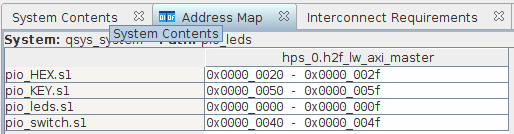
\includegraphics[scale=0.6]{./images/address_map.png}
\captionof{figure}{Laboratoire 2 : Address map}
\par
Le choix des offsets ci-dessus vient à la base d'un problème de compréhension. J'avais choisi ces offsets en fonction des adresses correspondantes dans le memory layout fournit dans le document "DE1-SoC\_Computer\_ARM.pdf". Si cela n'apporte pas de problème en tant que tel, il faut tout de même noter que j'aurais pu en choisir d'autres, en faisant en sorte qu'ils soient contiguës par exemple.

